\documentclass[a4paper, 11pt]{article}
\usepackage{/Users/fgu/dev/projects/dotfiles/latex/paper}
\bibliography{/Users/fgu/dev/projects/dotfiles/latex/fabib}
\onehalfspacing

\newcommand{\figdir}{../../output/figures}
\newcommand{\tabdir}{../../output/tables}

\title{\textbf{Evaluation\footnote{This research was supported by Economic and Social Research Council grant number ES/V004867/1. WBS ethics code: E-414-01-20.}}}

\author{
    Fabian Gunzinger \\ Warwick Business School
    \and
    Neil Stewart \\ Warwick Business School
}

\date{\today}

\begin{document}

\maketitle
% % !TEX root = ../entropy.tex

\begin{abstract}
    ...
\end{abstract}


\tableofcontents
\newpage

% % !TEX root = ../entropy.tex

\section{Introduction}%
\label{sec:introduction}

This paper documents variations in spending profiles and payments into
emergency savings for a large set of users of a financial management app
and shows that spending profiles predict emergency savings.

We define emergency savings as inflows into savings accounts. These savings
will be made up of savings for particular goals -- a new car, a holiday, a
wedding -- and savings directed towards building up a buffer for financial
emergencies. Because in our data we cannot distinguish between these two cases,
we refer to all of them as emergency savings.\footnote{MDB allows users to
    create custom tags and some users use them to indicate the intended use for
    their savings transactions (e.g. ``wedding'', ``holidays''). But only a very
small number of transactions have such tags, and we do not pursue this
further.} These short-term savings are distinct from long-term savings aimed to
build up funds for retirement, either through individually owned pension and
investment vehicles or employer-linked pension schemes. Both kinds of saving
are important for financial well-being, yet while there is a large literature
on pension savings, little is known about how people save for the
short-term.\footnote{Well-documented behavioural biases that help explain
    undersaving for pensions are, among others, present bias
    \citep{laibson1997golden, laibson2019intertemporal}, inertia
    \citep{madrian2001power}, over-extrapolation \citep{choi2009reinforcement},
    and limited self-control and willpower \citep{thaler1981economic,
    benhabib2005modeling, fudenberg2006dual, loewenstein2004animal,
gul2001temptation}. One danger of viewing low savings mainly as a result of
behavioural biases is that while these biases likely do play some role and
designing environments and tools to help correct them are thus part of the
solution, it is at least conceivable that this is an area where the focus on
behaviour-level solutions distracts from an effort to find more effective
society-level solutions, a danger inherent in behavioural science research
convincingly highlighted in \citet{chater2022frame}: if the main problem is
that many people are unable to earn enough to save, then the effectiveness of
helping them manage their low incomes more effectively pales in comparison with
efforts to help them earn more.}

Studying the determinants of emergency savings is important because around a
quarter of adults in the UK and the US are unable to cover irregular expenses
like car and medical bills: In the UK, 25 percent of adults would be unable to
cover an unexpected bill of \pounds300 \citep{philipps2021supporting}, while in
the US, about 30 percent would be unable to cover a \$400 bill
\citep{fed2022economic}. Similarly, resarch in the UK has shown that having
\pounds1000 in savings reduces by more than half a household's chances of
falling into debt that leads to financial problems
\citep{philipps2021supporting}.


Studying spending profiles is of interest because:
\begin{itemize}

    \item Our understanding of how people spend their money is based on survey
        data.

    \item Large-scale transaction-level data offers the possibility to study
        spending behaviour based on real-time data that are automatically
        collected for a large number of users. Such data has only become
        available ver recently and have not, thus far, been used to investigate
        systematically how people spend their money.

    \item Research in psychology suggests that disorder is maladaptive and
        associated with a range of negative outcomes such as impaired executive
        function \citep{vernon2016predictors}, lower cognitive inhibition
        \citep{mittal2015cognitive}, and activation of anxiety-related neural
        circuits \citep{hirsh2012psychological}. In the study of human
        behaviour, more chaotic behaviour has been found to predict the a
        higher number of visits to and higher spend in supermarkets
        \citep{guidotti2015behavioral}, higher calorie intake
        \citep{skatova2019those} and financial distress
        \citep{muggleton2020evidence}.

\end{itemize}


We hypothesise that less predictable spending patterns are associated with a
lower probability for making payments into emergency savings accounts. Possible
channels:
\begin{itemize}
    \item Disorder (personal life or environment): leads to more impulsive
        shopping behaviour and makes forgetting to save more likely.

    \item Scarcity: life challenges focus attention away from deliberate
        shopping, causing hore impulse purchases, and make fortetting to save
        more likely.
\end{itemize}



What we do: 
\begin{itemize}

    \item Systematically documenting emergency savings patterns.

    \item Systematically documenting variation in spending profiles.

    \item Showing that unpredictability in spending profiles is
        associated with lower emergency savings.

\end{itemize}


Contribution to literatures:
\begin{itemize}

    \item Understanding emergency savings behaivour (nest, aspen
        reports), \citep{sabat2019rules} for sources on short-term savings
        literature, \citet{colby2013savings} for lit on savings goals.  See
        \citet{colby2013savings} has useful literature review on short-term
        savings and suggests that subgoals can increase willingness to forego
        short-amounts in the present because they move the reference point in a
        prospect-theory framework. \citet{philipps2021supporting} present
        results from an employer-linked initiative that offers employees to
        have a portion of their salary automatically transferred into a savings
        pot. Policy literature: \citep{can2019improving,cfpb2017financial,
        mps2018building}. Older literature:Savings lit:
        \citet{lunt1991psychological, oaten2007improvements}

    \item Understanding effect of behavioural entropy - eliciting
        useful personality characteristics from large-scale data.

    \item Use of high-frequency transaction data (itself a
        sub-literature of use of newly available large-scale datasets).

\end{itemize}


\section{Introduction}%
\label{sec:introduction}


% % !TEX root = ../entropy.tex

\section{Methods}%
\label{sec:methods}



\subsection{Model specification}%
\label{sub:model_specification}



\begin{equation}
    s_{i,t} = \alpha_i + \lambda_t + \beta H_{i,t} + \zeta X_{i,t} + \epsilon_{i,t}
\end{equation}

$s_{i,t}$ is individual $i$'s savings rate in month $t$, calculated as the
total inflow of funds in month $t$ into all savings accounts held by $i$,
divided by $i$'s estimated monthly income.

The vector of control variables, $X_{i,t}$, contains the monthly spend for each
spending category, total monthly spend across all categories, and annual income.





\section{Methods}%
\label{sec:data}

\subsection{Outcomes}%
\label{sub:outcomes}

Our main outcome variable is savings as a proportion of monthly income, where
we measure savings as the sum of all savings account inflows. For a more
nuanced understanding of how app use affects savings we also consider net-savings --
total savings account inflows minus outflows -- as a proportion of monthly
income to see whether a willingness to save more might be offset by a (later)
need to withdraw funds, and a dummy variable for whether a user has any savings
account inflows in a given month to see whether the app helps users save at
all. To investigate possible channels, we consider total spend, highly
discretionary spend, banking charges, the total amount of borrowing, as well as
payday borrowing, all as proportion of monthly income. We think of these
additional outcomes as exploratory and do not make any adjustments for multiple
hypothesis testing.\footnote{For a recent game-theoretically motivated
discussion of when and how to correct for multiple hypothesis testing, see
\citet{viviano2021should}.}

An alternative approach, based on \citet{anderson2008multiple}, would be to
group outcomes into ``savings'', ``spending'', ``borrowing'', and ``fees'', and
consider them as different dimensions of a latent variable of interest which we
might call ``financial management skills''. We do not do that for two reasons:
first and foremost, because we think it is natural to think of the amount saved
as the ultimate outcome and of other outcomes as providing a more nuanced
understanding of savings behaviour or as suggesting possible channels through
which app use affects savings. Thinking of savings as the main goal is also
reflected in Money Dashboard's main promise, which is to help users spend less
and save more, as shown in Figure~\ref{fig:mdb_website}. Second, as pointed out
in \citet{carlin2017fintech}, incurring overdraft fees is not an unambiguous
sign of a financial mistake, as the opportunity to go into overdraft confers a
benefit to the consumer.\footnote{For further discussions on fees, see
\citet{jorring2020financial, stango2009consumers}.}


\subsection{Analysis plan (temp)}%
\label{sub:analysis_plan_temp_}
\begin{itemize}
    \item Show descriptive results (simple fig of behaviour change pre-post)

    \item Follow sakaguchi2022default (i.d. use dynamic TWFE DiD with synthetic
        control), but use sun2022estimating and the
        fixest implementation thereof to account for dynamic TWFE contamination
        issue
        \href{https://lrberge.github.io/fixest/articles/fixest_walkthrough.html#staggered-difference-in-differences-sun-and-abraham-2020}{paper}

    \item Main results: Figure and associated table akin to
        sakaguchi2022default Figure 2 and Table 6.

    \item Subgroup analysis: same Fig an Tab as in main analysis, but with line
        for each subgroup. One figure for each of: gender, generations, income
        terciles, per-adoption average savings tercile (inspired by
        \citet{carlin2017fintech}, see Fig 5 and Table 4).

    \item Robustness check with 12 and 18 month data windows.

\end{itemize}

\subsection{Difference-in-difference}%
\label{sub:difference_in_difference}

Control group design:
\begin{itemize}

    \item We only have data for a self-selected group of people who choose to
        use Money Dashboard. By virtue of signing up to an app that helps them
        manage their money, these users are different from those who don't sign
        up. As a result, we are unable to answer the question of whether use of
        Money Dashboard helps the average person in the population as a whole
        save more.\footnote{One way to get closer to that answer is to
            re-weight our sample on observable demographic variables so as to
            match the UK population as a whole. But our sample differs from the
            population as a whole both is ways that are observable (demographic
            variables) and unobservable (self-awareness that they need help
            managing their money, cognitive resources to engage with the app,
            motivation to do so). Re-weighting would only help us deal with the
        first of these.} Instead, we are answering the question whether Money
        Dashboard succeeds in helping its \textit{users} save more.

    \item Money Dashboard can access up to three years of historic data for
        each account a user links to their account.

    \item Each user for whom we have sufficient data thus serves as both a
        treatment unit and a potential control unit.

    \item We use a difference-in-differences design to estimate the effect of
        app use. Because we do not have a separate control group, we use the
        per-signup data of Money Dashboard users as control periods and use
        matching to find comparable control user for each tretment user.

    \item To perform the matching, we proceed as follows:

    \item For treatment units, we select data for six months before and after
        signup, where the month of the signup is treated as the first of the
        six after-signup months. For each user, we then calculate the mean
        value of each covariate for the pre-signup period.

    \item We construct potential control units as all 12-month data windows we
        observe before signup, and for each potential control unit calculate
        the mean value of each covariate for the first six months.

    \item We use matching proceedure introduced in \citet{ho2007matching} and
        implemented in the \textit{MatchIt} R-package \citep{stuart2011matchit} to
        find most similar comparison unit for each treatment unit.

    \item Matching method:

\end{itemize}

Estimating treatment effects
\begin{itemize}

    \item Our estimate is the ATT, not the ATE. 

    \item First, we present pre and post signup comparisons without matching
        (i.e. control group is user pre-signup).

    \item Second, we present (static) pre-post using matched comparisons.

    \item Third, we present dynamic pre-post using matched comparisons. Need to
        think about how this relates to \citet{sun2021estimating}, who propose
        an unbiased estimator for dynamic two-way FE event study designs. I
        think our analysis nests theirs, since we might still want to include
        fixed and time effects, though I need to think about this. (Reason to
        do so: we won't be able to match perfectly, so including user and time
        fixed effects to control for unit and time invariant variation still
        seems useful).

    \item As alternative to matching, consider synthetic controls for
        disaggregated data \citep{abadie2021penalized}.

\end{itemize}


% % !TEX root = ../entropy.tex

\section{Spending profiles predict emergency savings}%
\label{sec:results}

Table~\ref{tab:reg_has_inflows_main} shows the effect of entropy on the
probability of having emergency savings. Columns (1)-(3) show results for
unsmoothed entropy based on 9 categories, 48 categories, and merchant names,
respectively. Columns (4)-(6) results for smoothed entropy based on the same
variables. All models include user and year-month fixed effects, and standard
errors are clustered at the user-level. Confidence intervals are shown in
brakets.

\input{\tabdir/reg_has_inflows_main.tex}

Results for unsmoothed entropy suggest that a one unit increase in entropy is
associated with an increase in the probability of a user making at least one
transfer into their savings accounts of between 1.5 and 2.7 percentage points
-- an effect up to two times larger than that of a \pounds1000 increase in
monthly income.

Conversely, the effect for unsmooth entropy is smaller in magnitude but runs in
the reverse direction: a one-unit increase in the smoothed entropy score is
associated with a reduction in the probability of transferring money into
savings account of between 0.4 and 1.6 percentage points -- an effect that, in
absolute magnitude, is about equal to that of a \pounds1000 increase in monthly
income.

Overall, then, the effect of entropy in spending profiles is statistically and
economically significant, and robust across different definitions. In other
words, the scores seem to pick up a feature of the spending distribution that
is predictive of savings behaviour.

But how can we account for the opposite sign for smoothed and unsmoothed
entropy scores? We don't have the answer to this yet... 


\subsection{Effect of financial resilience}%
\label{sub:effect_of_financial_resilience}




If we think that it is scarcity that causes the relationship between
unpredictable spending behaviour and savings, then we would expect the effect
to be strongest for people with the lowest incomes, since they are more prone
to face financial shocks they find difficult to meet. The results below support
such an interpretation: the effect of both unsmoothed and smoothed entropy on
the probability of making a savings transaction is largest in magnitude for
users in the first income quintile.

In these regressions, we do not control for whether a user has income in in a
given month, since for all but the group in the first income quintile, this
will always be the case.


\begin{table}[htbp]
   \centering
   \tiny
   \begin{threeparttable}[b]
      \caption{\label{tab:reg_has_inflows_entropy_tag_spend_z_inc_quint} Effect of entropy on P(has savings) by income quintile}
      \begin{tabular}{lccccc}
         \tabularnewline \midrule \midrule
         Model:             & (1)             & (2)             & (3)            & (4)            & (5)\\  
         Income quintile:   & 1               & 2               & 3              & 4              & 5 \\   
         \midrule
         \emph{Variables}\\
         Entropy (48 cats)  & 0.033$^{***}$   & 0.019$^{***}$   & 0.017$^{***}$  & 0.016$^{***}$  & 0.018$^{***}$\\   
                            & [0.028; 0.039]  & [0.013; 0.025]  & [0.011; 0.023] & [0.010; 0.022] & [0.012; 0.025]\\   
         Month spend        & 0.010$^{***}$   & 0.007$^{***}$   & 0.008$^{***}$  & 0.007$^{***}$  & 0.006$^{***}$\\   
                            & [0.009; 0.011]  & [0.006; 0.008]  & [0.006; 0.009] & [0.006; 0.008] & [0.005; 0.007]\\   
         Month income       & 0.015$^{***}$   & 0.010$^{***}$   & 0.012$^{***}$  & 0.013$^{***}$  & 0.008$^{***}$\\   
                            & [0.012; 0.019]  & [0.004; 0.017]  & [0.005; 0.019] & [0.008; 0.019] & [0.007; 0.010]\\   
         Income variability & -0.000          & 0.001           & 0.002$^{***}$  & 0.001$^{**}$   & -0.000\\   
                            & [-0.001; 0.001] & [-0.000; 0.002] & [0.001; 0.004] & [0.000; 0.002] & [-0.001; 0.001]\\   
         \midrule
         \emph{Fixed-effects}\\
         User               & Yes             & Yes             & Yes            & Yes            & Yes\\  
         Year-month         & Yes             & Yes             & Yes            & Yes            & Yes\\  
         \midrule
         \emph{Fit statistics}\\
         Observations       & 223,462         & 215,151         & 208,417        & 201,319        & 195,378\\  
         R$^2$              & 0.59138         & 0.58949         & 0.58354        & 0.58212        & 0.57162\\  
         Within R$^2$       & 0.00535         & 0.00180         & 0.00211        & 0.00191        & 0.00271\\  
         \midrule \midrule
         \multicolumn{6}{l}{\emph{Clustered (User) co-variance matrix, 95\% confidence intervals in brackets}}\\
         \multicolumn{6}{l}{\emph{Signif. Codes: ***: 0.01, **: 0.05, *: 0.1}}\\
      \end{tabular}
   \end{threeparttable}
\end{table}



\input{\tabdir/reg_has_inflows_entropy_tag_spend_sz_inc_quint.tex}


\begin{table}[htbp]
   \centering
   \tiny
   \begin{threeparttable}[b]
      \caption{\label{tab:reg_has_inflows_entropy_tag_spend_z_inc_var_quint} Effect of entropy on P(has savings) by income variability quintile}
      \begin{tabular}{lccccc}
         \tabularnewline \midrule \midrule
         Model:                       & (1)             & (2)            & (3)             & (4)             & (5)\\  
         Income variability quintile: & 1               & 2              & 3               & 4               & 5 \\   
         \midrule
         \emph{Variables}\\
         Entropy (48 cats)            & 0.020$^{***}$   & 0.014$^{***}$  & 0.022$^{***}$   & 0.028$^{***}$   & 0.021$^{***}$\\   
                                      & [0.014; 0.026]  & [0.008; 0.020] & [0.016; 0.028]  & [0.022; 0.034]  & [0.015; 0.027]\\   
         Month spend                  & 0.008$^{***}$   & 0.008$^{***}$  & 0.007$^{***}$   & 0.007$^{***}$   & 0.007$^{***}$\\   
                                      & [0.007; 0.009]  & [0.007; 0.009] & [0.006; 0.008]  & [0.006; 0.008]  & [0.006; 0.008]\\   
         Month income                 & 0.014$^{***}$   & 0.010$^{***}$  & 0.011$^{***}$   & 0.010$^{***}$   & 0.010$^{***}$\\   
                                      & [0.011; 0.017]  & [0.008; 0.012] & [0.010; 0.013]  & [0.009; 0.012]  & [0.009; 0.011]\\   
         Has income in month          & 0.092$^{***}$   & 0.076$^{***}$  & 0.064$^{***}$   & 0.055$^{***}$   & 0.067$^{***}$\\   
                                      & [0.073; 0.111]  & [0.056; 0.095] & [0.047; 0.081]  & [0.040; 0.070]  & [0.053; 0.081]\\   
         Income variability           & -0.001          & 0.006$^{**}$   & -0.000          & 0.000           & -0.004$^{**}$\\   
                                      & [-0.003; 0.001] & [0.001; 0.011] & [-0.004; 0.003] & [-0.001; 0.002] & [-0.007; -0.001]\\   
         \midrule
         \emph{Fixed-effects}\\
         User                         & Yes             & Yes            & Yes             & Yes             & Yes\\  
         Year-month                   & Yes             & Yes            & Yes             & Yes             & Yes\\  
         \midrule
         \emph{Fit statistics}\\
         Observations                 & 223,462         & 215,151        & 208,417         & 201,319         & 195,378\\  
         R$^2$                        & 0.61166         & 0.59951        & 0.59062         & 0.59379         & 0.63519\\  
         Within R$^2$                 & 0.00558         & 0.00398        & 0.00484         & 0.00579         & 0.00781\\  
         \midrule \midrule
         \multicolumn{6}{l}{\emph{Clustered (User) co-variance matrix, 95\% confidence intervals in brackets}}\\
         \multicolumn{6}{l}{\emph{Signif. Codes: ***: 0.01, **: 0.05, *: 0.1}}\\
      \end{tabular}
   \end{threeparttable}
\end{table}




\begin{table}[htbp]
   \centering
   \tiny
   \begin{threeparttable}[b]
      \caption{\label{tab:reg_has_inflows_entropy_tag_spend_sz_inc_var_quint} Effect of entropy on P(has savings) by income variability quintile}
      \begin{tabular}{lccccc}
         \tabularnewline \midrule \midrule
         Model:                       & (1)              & (2)              & (3)              & (4)              & (5)\\  
         Income variability quintile: & 1                & 2                & 3                & 4                & 5 \\   
         \midrule
         \emph{Variables}\\
         Entropy (48 cats, smooth)    & -0.019$^{***}$   & -0.020$^{***}$   & -0.017$^{***}$   & -0.022$^{***}$   & -0.024$^{***}$\\   
                                      & [-0.024; -0.015] & [-0.024; -0.016] & [-0.021; -0.013] & [-0.026; -0.018] & [-0.028; -0.019]\\   
         Month spend                  & 0.007$^{***}$    & 0.007$^{***}$    & 0.006$^{***}$    & 0.006$^{***}$    & 0.006$^{***}$\\   
                                      & [0.006; 0.008]   & [0.006; 0.008]   & [0.005; 0.008]   & [0.005; 0.007]   & [0.005; 0.007]\\   
         Month income                 & 0.014$^{***}$    & 0.010$^{***}$    & 0.011$^{***}$    & 0.010$^{***}$    & 0.010$^{***}$\\   
                                      & [0.011; 0.017]   & [0.008; 0.012]   & [0.009; 0.013]   & [0.009; 0.012]   & [0.009; 0.011]\\   
         Has income in month          & 0.093$^{***}$    & 0.075$^{***}$    & 0.064$^{***}$    & 0.056$^{***}$    & 0.066$^{***}$\\   
                                      & [0.074; 0.112]   & [0.055; 0.094]   & [0.047; 0.081]   & [0.040; 0.071]   & [0.052; 0.081]\\   
         Income variability           & -0.001           & 0.005$^{**}$     & -0.000           & 0.000            & -0.004$^{**}$\\   
                                      & [-0.003; 0.001]  & [0.001; 0.010]   & [-0.004; 0.003]  & [-0.001; 0.002]  & [-0.006; -0.001]\\   
         \midrule
         \emph{Fixed-effects}\\
         User                         & Yes              & Yes              & Yes              & Yes              & Yes\\  
         Year-month                   & Yes              & Yes              & Yes              & Yes              & Yes\\  
         \midrule
         \emph{Fit statistics}\\
         Observations                 & 223,462          & 215,151          & 208,417          & 201,319          & 195,378\\  
         R$^2$                        & 0.61181          & 0.59979          & 0.59070          & 0.59394          & 0.63550\\  
         Within R$^2$                 & 0.00597          & 0.00466          & 0.00502          & 0.00614          & 0.00864\\  
         \midrule \midrule
         \multicolumn{6}{l}{\emph{Clustered (User) co-variance matrix, 95\% confidence intervals in brackets}}\\
         \multicolumn{6}{l}{\emph{Signif. Codes: ***: 0.01, **: 0.05, *: 0.1}}\\
      \end{tabular}
   \end{threeparttable}
\end{table}






\section{Results}%
\label{sec:results}

\subsection{Descriptive analysis}%
\label{sub:descriptive_analysis}

\subsection{Difference-in-difference analysis}%
\label{sub:difference_in_difference_analysis}

\subsection{Subgroups}%
\label{sub:subgroups}

To analyse which groups benefit most from adopting Money Dashboard, we split
our sample by gender, generation, income quartiles, and pre-adoption savings
behaviour.

We define generations as follows: boomers were born between 1946 and 1964, Gen
X between 1965 and 1980, Millennials between 1981 and 1996, and Gen Z after
1997.\footnote{Based on age ranges provides by
    \href{https://www.beresfordresearch.com/age-range-by-generation/}{Beresford
Research}.}

\subsection{Alternative window lengths}%
\label{sub:alternative_window_lengths}

% % !TEX root = ../entropy.tex

\section{Discussion}%
\label{sec:discussion}

\edit{Ignore this section for now. Below are just notes.}
There are a number of alternative ways to characterise spend profiles. We could
calculate profiles based on the distribution of transaction values rather than
counts. We could also calculate profiles based on inter-temporal rather than
intra-temporal distributions, focusing on consistency of purchasing behaviour
over time rather than on predictability at any given time
\citep{krumme2013predictability}. Further, we could focus on time-based rather
than category-based measures, focusing, for instance, on whether purchases of
the same type tend to occur on the same day of the week
\citep{guidotti2015behavioral}. Finally, one could also create composite
measures based on principal component analysis, an approach used in
\citet{eagle2010network}. We leave these extensions for future research.


\section{Discussion}%
\label{sec:discussion}







\newpage
\printbibliography
\newpage

% % !TEX root = ../entropy.tex

\section{Interpreting entropy}%
\label{sec:interpreting_entropy}

To see how we can interpret entropy as the predictability of a user's spending behaviour, it is useful to have a more complete
understanding of Equation~\ref{equ:entropy}. The building blocks of entropy is
the information content of a single event. The key intuition
\citet{shannon1948mathematical} aimed to capture was that learning of the
occurrence of a low-probability event is more informative than learning of the
occurrence of a high-probability event. The information of an event $I(E)$ is
thus inversely proportional to is probability $p(E)$. One way to capture this
would be to define the information of event E as $I(E) = \frac{1}{p(E)}$. Yet
this implied that an event that is certain to occur had information 1, when it
would make sense to have information 0. To remedy this (and also satisfy
additional desireable characteristics of an information function), Shannon
proposed using the log of the expression. Hence, the information of event E,
often called \textit{Shannon information}, \textit{self-information}, or just
\textit{information}, is defined as:

\begin{equation}
    I(E) = log\left(\frac{1}{p(E)}\right) = -log(p(E)).
\end{equation}

The choice of the base for the logarithm varies by application and determines
the units: base 2 means that information is expressed in bits; the natural
logarithm, another popular choice, expresses information in \textit{nats}.

Entropy, often called \textit{Information entropy}, \textit{Shannon entropy},
or just \textit{entropy}, is the information of a random variable, $X$, and
captures the expected amount of information of an event drawn at random from
the probability distribution of the random variable. It is calcualted as:

\begin{equation}
    H(X) = -\sum_x p(x) \times log(p(x)) = \sum_x p(x)I(x) = \mathbb{E} I(x).
\end{equation}

For a single event, the key intution was that the less likely an event, the
more information is conveyed when it occurs. The related idea for distributions
is similar: the less skewed a distribution of a random variable, the less
certain the realised value of a single draw from the distribution, the higher
is entropy - the maximum entropy distribution is the uniform distribution.


\section{Entropy components}%
\label{sec:entropy_components}

Figure~\ref{fig:entropy_components} shows the empirical relationship with our
48-categories-based unsmoothed entropy variable and these three
components.\footnote{To highlight the main features of the relationships we
have trimmed the component values at the 95th percentile.} We can see that for
the values we observe in the dataset, entropy increases monotonically in the
number of unique spending categories with positive frequency counts, has no
clear relationship with the standard deviation of those counts, and increases
in the number of total spending transactions up to about 175 transaction,
before being increasingly determined by other elements thereafter.

\begin{figure}[ht]
    \centering 
    \caption{Correlation of entropy with its components}
    \label{fig:entropy_components}
    \includegraphics[width=.32\textwidth]{\figdir/scatter_entropy_nunique_tag_spend.pdf}
    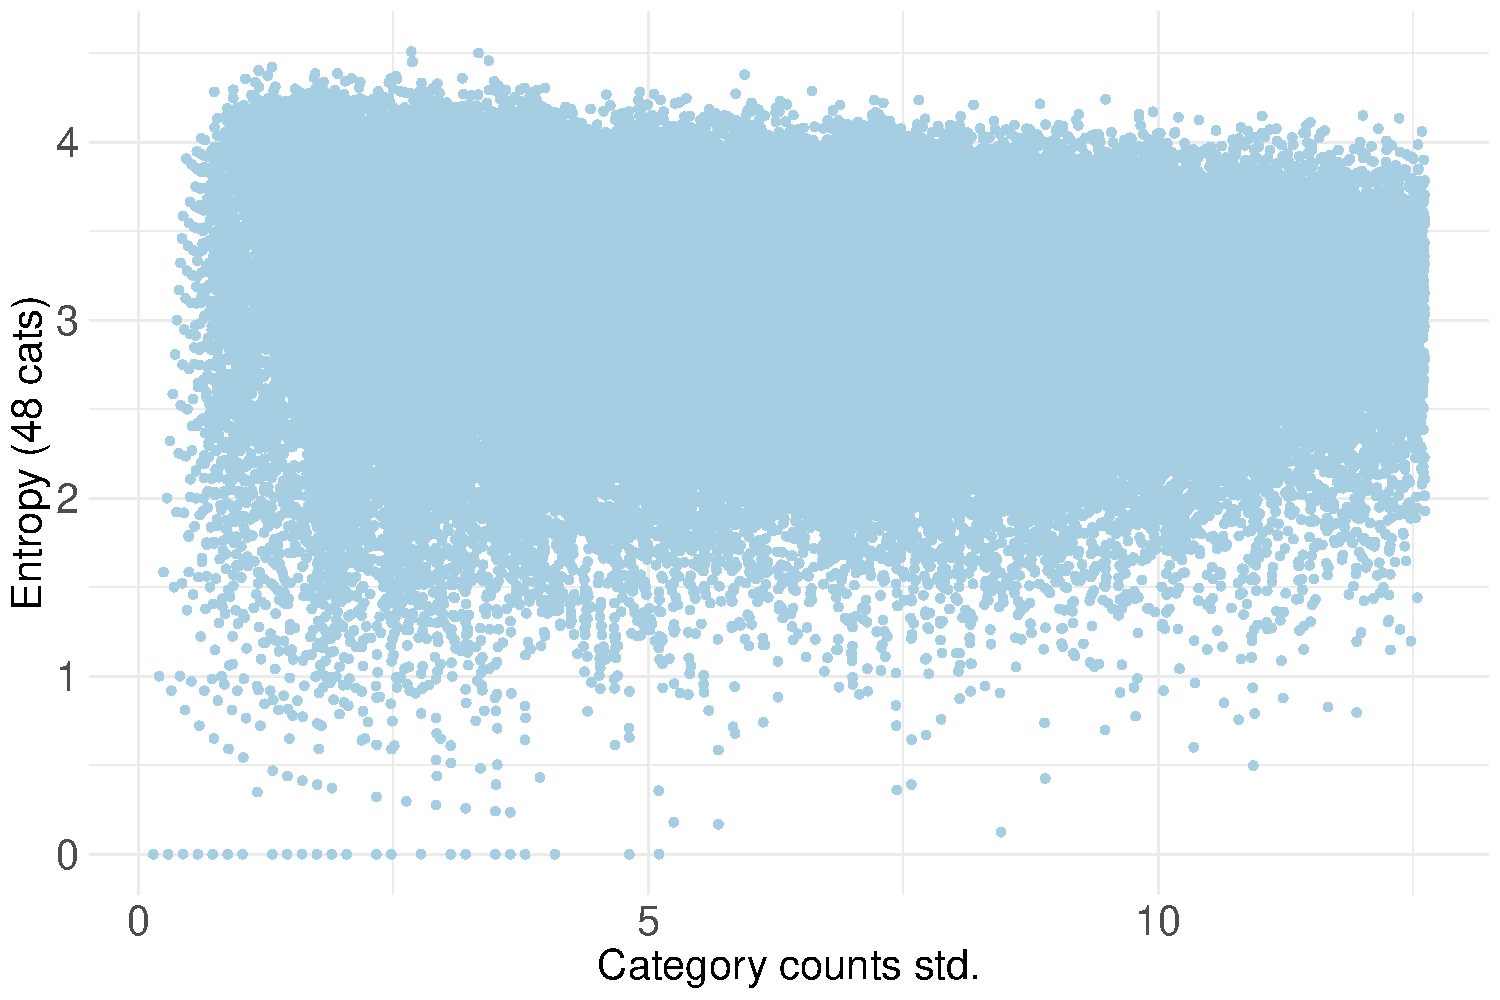
\includegraphics[width=.32\textwidth]{\figdir/scatter_entropy_std_tag_spend.pdf}
    \includegraphics[width=.32\textwidth]{\figdir/scatter_entropy_txns_count_spend.pdf}
    \fignote{\textwidth}{Correlation of 48-categories-based unsmoothed entropy
    with its three main components: the number of unique spending categories
with positive frequency counts (left), the standard deviation of those
frequency counts (middle), and the number of total spend transactions (left).}
\end{figure}


\section{Effect of smoothing on entropy}%
\label{sec:effect_of_smothing_on_entropy}

\begin{figure}[ht]
    \centering 
    \caption{Effect of smoothing on entropy}
    \label{fig:scatter_facets_txns_count_spend_q}
    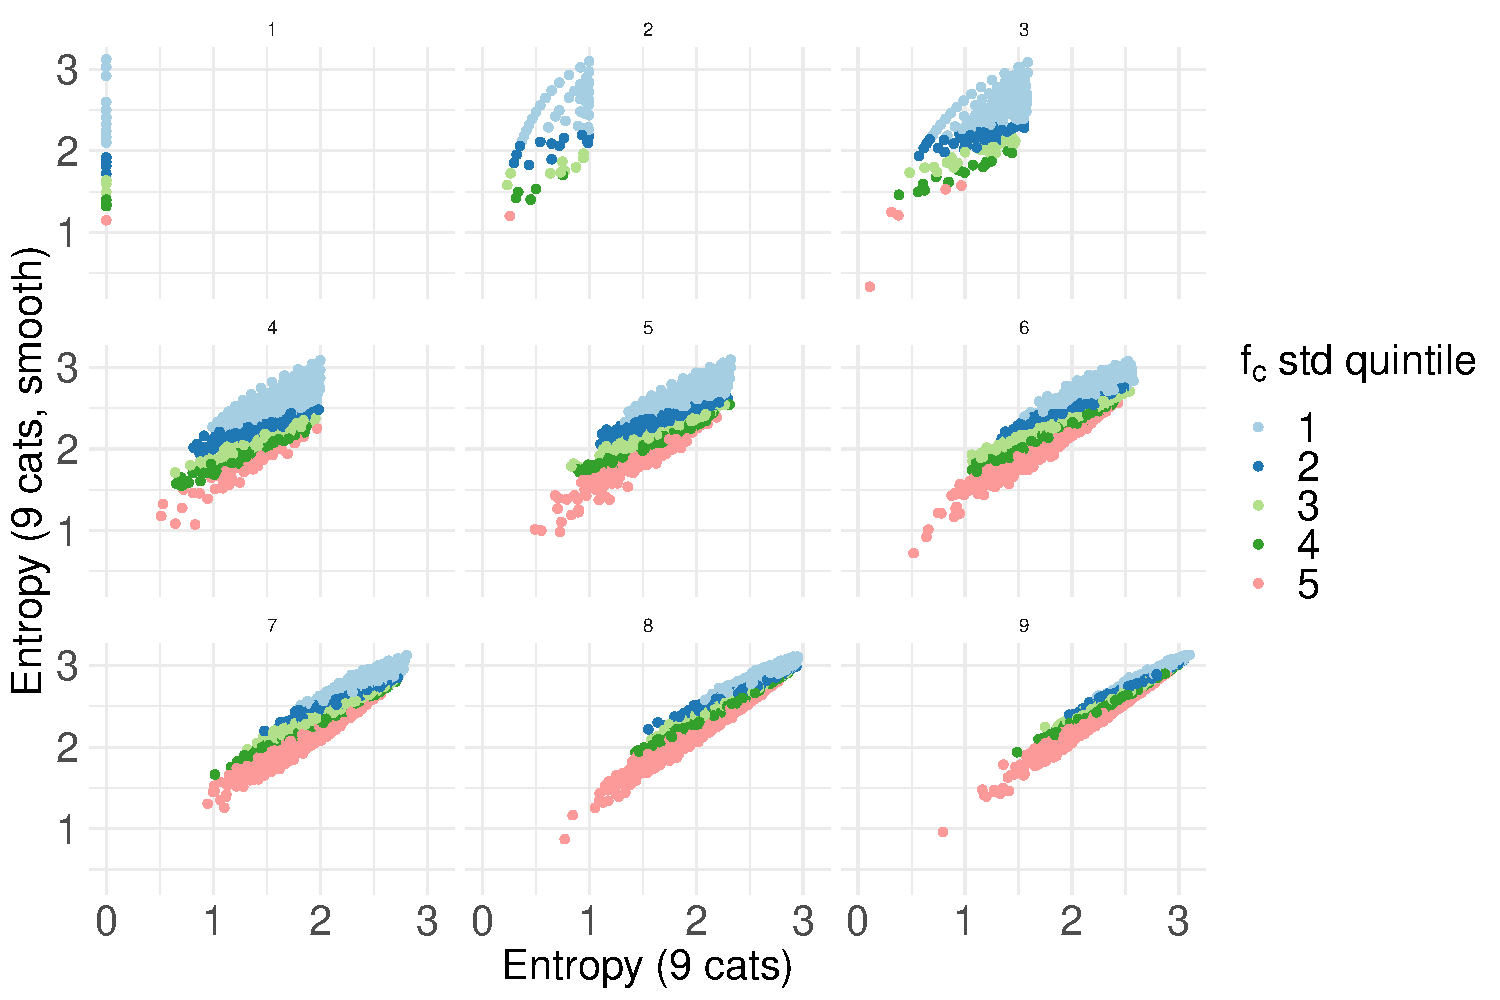
\includegraphics[width=\textwidth]{\figdir/scatter_facet_std_tag_q.pdf}
    \fignote{\textwidth}{Percentile ranks of 9-category-based unsmoothed and
    smoothed entropy separated by the number of categories with positive
frequency counts. White reference lines indicate equal percentile ranks.
Colours indicate the quintile of the total number of spending transactions.}
\end{figure}


\appendix

\section{Money Dashboard application}%
\label{sec:money_dashboard_application}

\begin{figure}[htpb]
    \centering
    \caption{Money Dashboard website screenshot}%
    \includegraphics[width=0.8\linewidth]{mdb_website}
    \label{fig:mdb_website}
\end{figure}
\fignote{\textwidth}{Screenshot from the top of the Money Dashboard website, at
\href{https://www.moneydashboard.com}{moneydashboard.com}, accessed on 29 April
2022.}

\end{document}
